%Approach

\section{Describing Co-Evolution}
\label{sec:approach}

The objective of this work is to obtain a consolidated view of changes occurring to features and their implementation.
This information is meant to be used for further analysis, and should capture the most relevant aspects of the changes regarding 
features and their evolution in the different spaces.
In this section, we present the meta-model we use to describe feature-related changes in the different artefacts,
and how we relate those changes to one-another.
We illustrate the usage of the model with an example of actual feature changes, affecting all spaces, extracted from release v3.11.
In this scenario, a developer commits a new driver for an ambient light sensor, ``APDS9300''.
The commit\footnote{commit id: 03eff7b60d} message for that change reads as follows:
\begin{verbatim}
iio: add APDS9300 ambilent light sensor driver
    
This patch adds IIO driver for APDS9300 ambient light sensor 
(ALS).
http://www.avagotech.com/docs/AV02-1077EN
    
The driver allows to read raw data from ADC registers or 
calculate lux value. It also can handle threshold interrupt.
\end{verbatim}

\subsection{FEVER Change Meta-model}

An overview of the FEVER change meta-model is shown in \figref{fig:patch_change_model}.
This overview highlights the different entities we use to describe what occurs in a commit, from a feature perspective.

The \textbf{commit} represents a commit in a version control system.
\textbf{Commit} entities are related to one another through the ``next'' relationship, 
capturing the sequence of changes over time.
Each \textbf{commit} ``touches'' a number of artefacts, and those changes are captured in \textbf{ArtefactEdit} entities.
The \textbf{commit} may affect any of the three spaces, leading to \textbf{SourceEdit} entities when code blocks related to features are modified,
\textbf{MappingEdit} entities when the mapping between feature and assets is affected, or finally
\textbf{FeatureEdit} entities when the variability model changes.

While the \textbf{ArtefactEdit} indicates a change to a file, \textbf{Source-, Mapping- and Feature- Edit} entities
are all representing the change related to individual features within those files.
We omitted the following relationship in the model for readability purposes:
\textbf{FeatureEdit}, \textbf{MappingEdit}, and \textbf{SourceEdit} entities are linked
to \textbf{ArtefactEdit} with a ``in'' relationship, pointing to the artefact in which the change took place.
This relationship is established at a file level. The details of the changes within that artefacts are contained 
in the associated \textbf{Edit} entity.
Finally, \textbf{Edit} entities pertaining to the same feature are linked together through \textbf{TimeLine} entity.
This grouping changes per feature using \textbf{TimeLine} entities is done over multiple commits (a complete release in our experiment).
Therefore, the \textbf{TimeLine} of a feature aggregates all changes that occurred to that feature over time \ie across multiple commits.

\begin{figure}[ht]
	\centering
	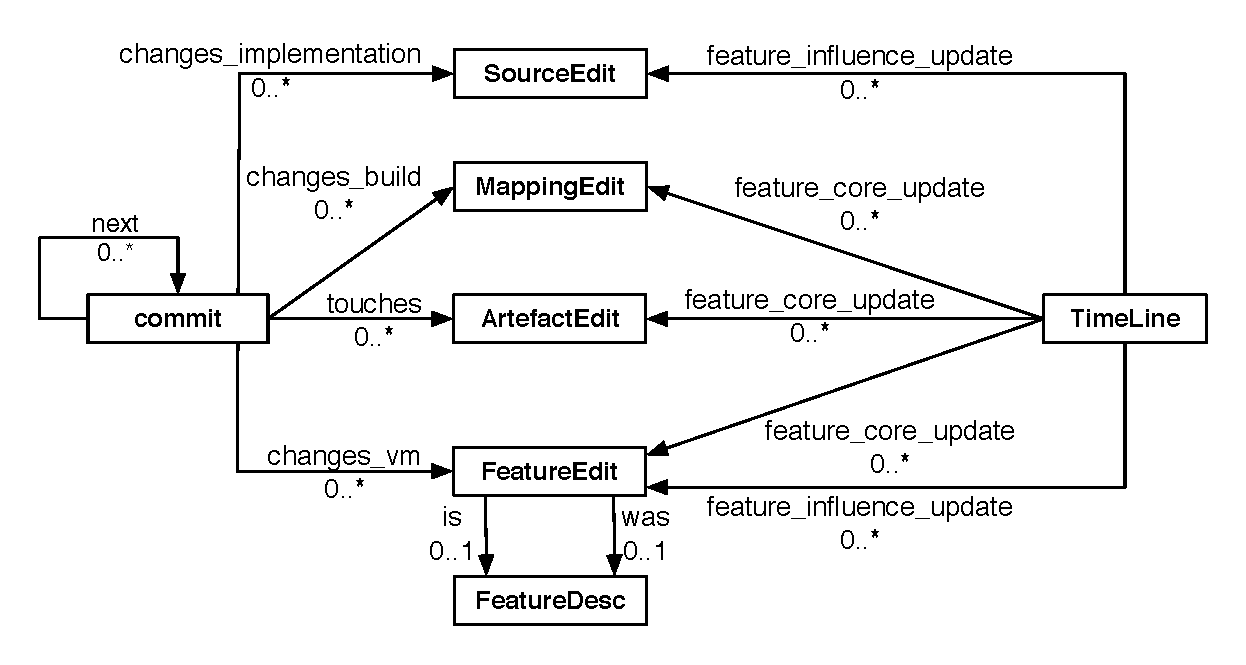
\includegraphics[scale=0.5]{change_model_new.eps}
	\caption{The FEVER change meta-model for feature-oriented change description}
	\label{fig:patch_change_model}
\end{figure}

For a commit in the repository we record the commit id (sha1) to link our data with the reference repository. 
We save the commit message which may contain information about the rationale of a change.
Finally, to keep track of who touches which feature, we record users-related information such as commiter and author of each commit.
\tabref{commit_attrs} summarizes the commit-related information stored in the FEVER database, examplified with the commit adding the 
``APDS9300'' feature.

\begin{table}[h]
\centering
\resizebox{\textwidth}{!}
{
\begin{tabular}{|l|l|l|}
\hline
Attribute 		& Details 										& Example\\
\hline
hash			& 10 first digits of the commit unique ID 		& 03eff7b60d \\
\hline
author			& author's name 								& Oleksandr Kravchenko\\
\hline
commiter 		& commiter's name 								& Jonathan Cameron\\
\hline
message 		& complete commit message, including sign-offs 	& iio: add APDS9300 ambilent light sensor driver (...)\\
\hline
time			& commit time 									& Sat Aug 03 19:40:37 CEST 2013\\
\hline
\end{tabular}
}
\caption{FEVER \textbf{Commit} entity attributes }
\label{commit_attrs}
\end{table}

\subsection{Variability Model Changes}

A \textbf{FeatureEdit} entity represents the change of one feature within the variability model performed in the context of a \textbf{commit}.
We are interested in the affected feature, as well as the change operation that took place (\textit{addition}, \textit{removal}, or \textit{modification} of an existing feature).
The \textbf{FeatureEdit} entity also points to a more complete description of the feature, \textbf{FeatureDesc} entities. 
\textbf{FeatureDesc} presents the feature as it ``was'' before the change (if existing)  and how it ``is'' after the edit operation (if existing).

In our example, the developer added a new feature, APDS9300, to the variability model.
The change that can be observed in the source control system is shown in \figref{fig:vm_change_diff}.

\begin{figure}[h]
\centering
	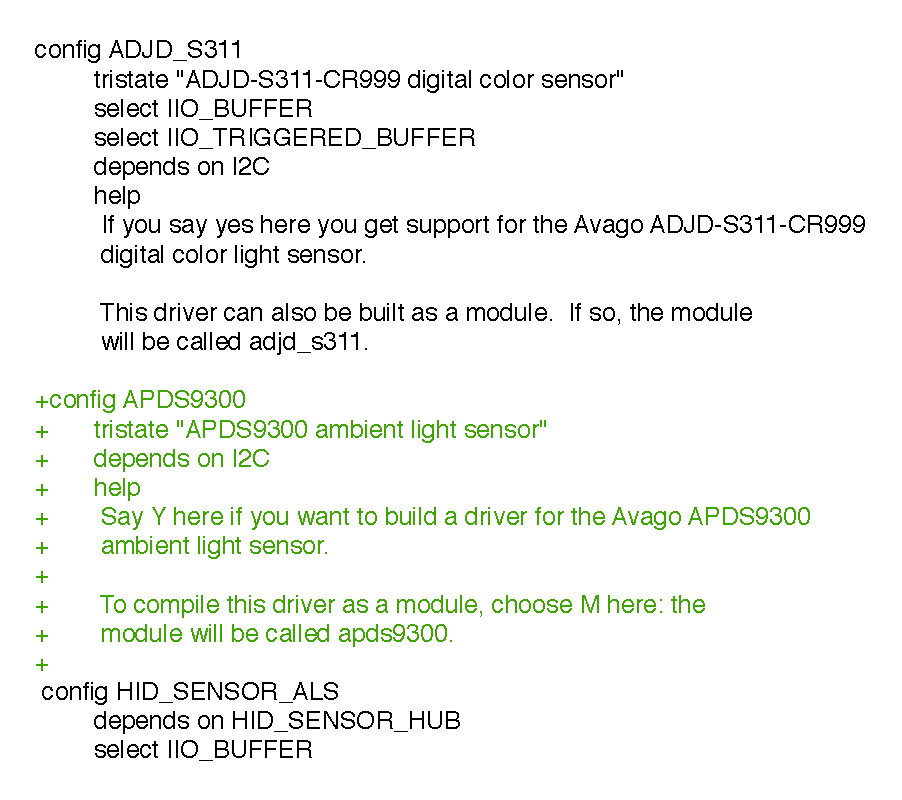
\includegraphics[scale=0.5]{VM_Diff_NewFeat.eps}
	\caption{Variability model change: addition of the feature APDS9300}
	\label{fig:vm_change_diff}
\end{figure}

The information recorded by FEVER on \textbf{FeatureEdit} entities are summarized in \tabref{featureedit_attrs}.
\begin{table}[h]
\resizebox{\textwidth}{!}
{
\centering
{
\begin{tabular}{|l|l|l|}
\hline
Attribute & Details & Example\\
\hline
name			& name of the touched feature & APDS9300 \\
\hline
change		& change operation affecting the feature  & ADDED\\
\hline
visibility	& feature visibility to user during configuration & visible\\
\hline
type &  type of the feature, defines its possible values & TRISTATE\\
\hline
\end{tabular}
}
}
\caption{FEVER \textbf{FeatureEdit} entity attributes }
\label{featureedit_attrs}
\end{table}

The possible values for the ``change'' attribute are: ``ADDED'', ``REMOVED'', or ``MODIFIED''.
The type attribute matches the configuration option type in the Kconfig language (``BOOLEAN'',``TRISTATE'', ``INT'', ``HEX'', or ``STRING'').
The feature is either ``visible'' or ``internal''.
Note that the type, and visibility information stored on the \textbf{FeatureEdit} entity correspond to the state of the feature after the edition takes place.
For additional information on the state of the feature before and after the change, one can refer to the \textbf{FeatureDesc} entities connected
to the \textbf{FeatureEdit} entity.

The \textbf{FeatureDesc} entity captures the information presented in \tabref{featuredesc_attrs}. 
\begin{table}[h]
\centering
\resizebox{\textwidth}{!}
{
\begin{tabular}{|l|l|l|}
\hline
Attribute & Details & Example\\
\hline
name			& name of the touched feature & APDS9300 \\
\hline
type 		& feature type &  TRISTATE \\
\hline
visibility 	& feature visibilty to the user during configuration & visible \\
\hline
depends on  & dependencies of the feature & I2C \\
\hline
selects 	    & the selected features & (none) \\
\hline
default values & default values, with conditions if any & (none) \\ 
\hline
\end{tabular}
}
\caption{FEVER \textbf{FeatureDesc} entity attributes}
\label{featuredesc_attrs}
\end{table}

For any feature change occurring at a variability model level, the change will be represented by a ``FeatureEdit'' entity, and at least one ``FeatureDesc'' entity in case of addition or removal,
and at most two in the case of the modification of an existing feature.


\subsection{Mapping Changes}

Regarding the evolution of the mapping, we are mainly interested in  the evolution of the mapping between feature and asset.
For this study, we consider the following types of assets: implementation artefacts, data artefacts, folders, and compilation flags.
The evolution of the mapping space is represented by \textbf{MappingEdit} entities characterized by:
the feature involved and the type of artefacts it is mapped to.
We describe the feature-mapping change operation (\textit{added}, \textit{removed}, or \textit{modified}),
referring to the association of a feature to any type of assets, and the change affecting the target within that mapping (\textit{added} or \textit{removed}).
Finally, if the asset is an artefact (file), then the change meta-model also includes the change to the artefact itself.
We can thus make the difference between a situation where a new mapping is introduced (\textit{addition} of a mapping with an \textit{added} target)
and an existing mapping being extended (\textit{modification} of a  mapping with an \textit{added} target).
If the asset is not an artefact (such as a folder or a compilation flag) the value of the ``artefact change'' attribute is set to ``NA''.

In our example, the developer adds a mapping between the newly created feature and a newly added file by
modifying an existing Makefile as shown in \figref{fig:mapping_change_diff}.
The information contained within the \textbf{MappingEdit} entity to represent this change are presented in \tabref{mapping_attrs}.

\begin{figure}[h]
\centering
	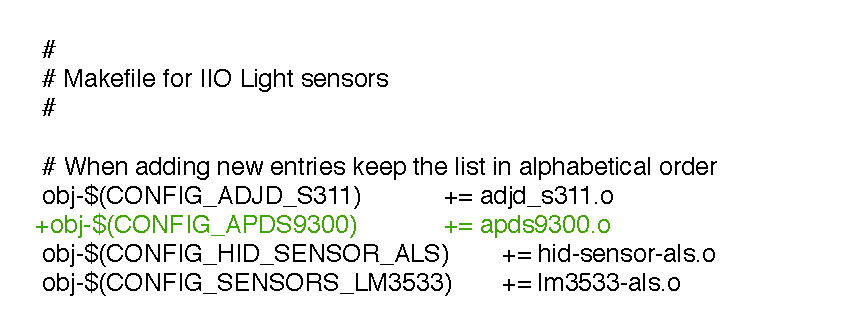
\includegraphics[scale=0.5]{Mapping_Diff_NewFeat.eps}
	\caption{Mapping change: introduction of a new association between feature and asset}
	\label{fig:mapping_change_diff}
\end{figure}

\begin{table}[h]
\centering
\resizebox{\textwidth}{!}
{
\begin{tabular}{|l|l|l|}
\hline
Attribute & Details & Example\\
\hline
type 		& element mapped to the asset &  FEATURE \\
\hline
feature		& name of the feature involved & APDS9300 \\
\hline
target		& target of the mapping & apds9300.o\\
\hline
target type	& type of the target (folder, flag, data, compilation unit)  & COMPILATION\_UNIT \\
\hline
mapping change  & change to the mapping of the feature  & ADDED \\
\hline
target change & change to the target entity within the feature's mapping & ADDED \\
\hline
artefact change	    & change to the artefact pointed to by the target & ADDED \\
\hline
\end{tabular}
}
\caption{FEVER \textbf{MappingEdit} entity attributes }
\label{mapping_attrs}
\end{table}

\subsection{Source Code Changes}

Feature related changes within source code, such as modifications to conditionally compiled blocks and feature references, 
are captured as \textbf{SourceEdit} entities.
Features in \#ifdef code block conditions and feature references within a given file are an indication 
that the behaviour of the feature mapped is configurable, and its exact behaviour is determined by other features.

Feature references are references to feature names within the code, meant to be replaced by the feature's value at compile-time.
Such references may only be \textit{added} or \textit{removed}.
In such cases, the \textbf{SourceEdits} entity contains the name of the affected feature and the change in question.

Conditionally compiled code blocks are identified by the conditions under which they will be included in the final product.
A change to such a block is represented by a \textbf{SourceEdit} containing the condition of the block, 
the change to the block itself (\textit{added, removed, modified}), and the change of the implementation within that block: 
\textit{added} if the code is entirely new, \textit{removed} if the whole block was removed, 
\textit{modified} when the changed block contains arbitrary edits, or finally \textit{preserved} if the code itself has not been touched.
An example of the code change is depicted in \figref{fig:src_change_diff}.

\begin{figure}[h]
\centering
	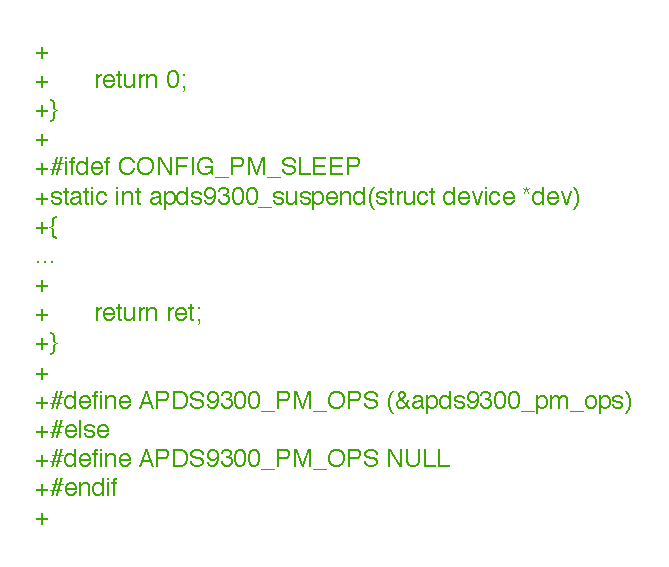
\includegraphics[scale=0.5]{Src_Diff_NewBlock.eps}
	\caption{Source change: addition of  conditionally compiled code blocks}
	\label{fig:src_change_diff}
\end{figure}

In our example, two code blocks are added. \tabref{sourceedit_attrs} presents the information we obtain
for the creation of the \textit{else} fragment of this change.
A similar entity is created for the first part of that new code block, the only different being the value of 
``interaction'' attribute which would reflect the condition of the first block, namely ``\textit{defined(CONFIG\_PM)}''

\begin{table}[h]
\centering
\resizebox{\textwidth}{!}
{
\begin{tabular}{|l|l|l|}
\hline
Attribute & Details & Example\\
\hline
Change 			& change to the code block itself, or the feature reference &  ADDED \\
\hline
Interaction		& presence condition of the block, or feature name for feature reference & !(defined(CONFIG\_PM\_SLEEP)) \\
\hline
Code Edit		& transformation of the code inside the changed block, ``null'' for references  & ADDED \\
\hline
\end{tabular}
}
\caption{FEVER \textbf{SourceEdit} entity attributes }
\label{sourceedit_attrs}
\end{table}

\subsection{TimeLines: Aggregating Feature Changes}

Changes pertaining to the same features are then aggregated into \textbf{TimeLine} entities.
A \textbf{TimeLine} entity aggregates all changes pertaining to a single feature in a number of commits - this includes
modification of artefacts mapped to the feature in question, FeatureEdit, MappingEdit or changes to conditionally compiled code blocks whose conditions refer to that feature.
For this study, we created \textbf{TimeLine} entities for entire releases.

We divide the types of changes that may affect a feature into two broad categories: 
\emph{core changes} and \emph{influence changes}.

A \emph{feature core update} indicates that the behaviour of the feature itself or its definition is being adjusted.
This comprises changes to the feature definition in the VM, changes to the mapping between the feature and assets,
and changes affecting assets mapped to that feature. 

A \emph{feature influence update} indicates that the feature is playing a role in the behaviour of another feature.
This occurs in two contexts: in the source code, as part of a \textbf{SourceEdit}, or in the variability model as 
part of a \textbf{FeatureEdit}. For instance, in the first case, Feature B plays a role in the implementation of A if we can find
an \#ifdef block refering to B in a source file mapped to Feature A. Similarly, Feature B plays a role in the definition of feature A
if Feature B appears anywhere in the definition of A in the variability model (as part of a default value, depends or select statement or any other attribute).

\figref{fig:commit_overview} depicts all entities and relationships used to describe the changes occurring in single commit
03eff7b60d. This is a partial view of the complete database. When fully expanded, the ``PM\_SLEEP'' \textbf{TimeLine} points to any
\textbf{Edit} entity which describe changes to the ``PM\_SLEEP'' feature across an entire release.
By navigating through those relationships, one can easily find what transformation occured on each feature and retrieve contextual information 
regarding this change.

\begin{figure}[htb]
	\centering
	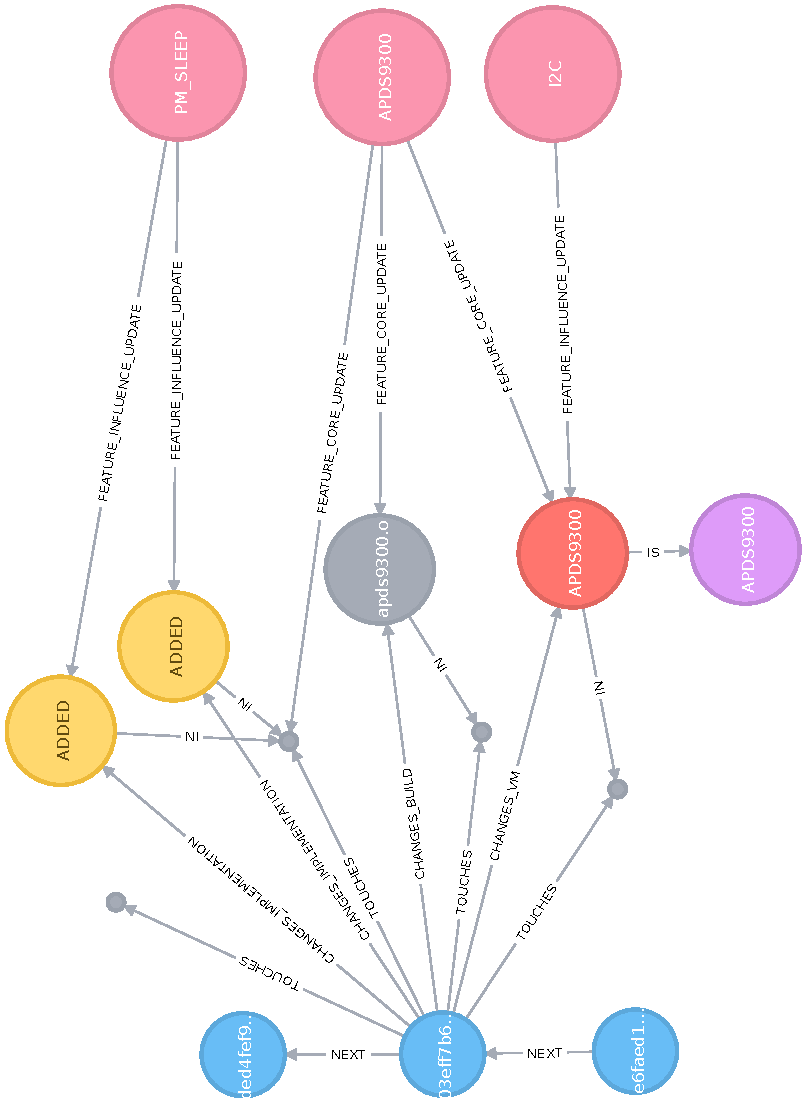
\includegraphics[scale=0.55,angle =-90, natwidth=450,natheight=500]{full_commit.pdf}
	\caption{FEVER representation of commit 03eff7b60d - all entities and relationships. For readability purposes, \textbf{ArtefactEdits} are
	represented by small unlabelled gray dots. From top to bottom, they represent edits to the following files: a documentation file, 
	the source file containing the  behavior of feature APDS9300, 
	the Makefile containing the new mapping, and the Kconfig file containing the new feature declaration.
	On the left hand side, we see three commits. On the right hand side, we see three feature \textbf{TimeLine} entities, one for each feature that was adjusted in the commit. In the middle, from top to bottom we see two source edits (labeled ``ADDED'') indicating that two \#ifdef blocks were added, one \textbf{MappingEdit}, labeled ``apds9300.o'', then a \textbf{FeatureEdit} entity indicating taht feature APDS9300 was changed, and a \textbf{FeatureDesc} entity containing a detailed description of how the feature ``is'' after the change.}
	\label{fig:commit_overview}
\end{figure}

\begin{sloppypar}

In \figref{fig:commit_overview}, three \textbf{TimeLine} entities are depicted in pink, on the right hand side of the diagram, annotated with the feature name.
The first one relates to the feature that was introduced. We can see that
the ``APDS9300'' node is connected to the \textbf{FeatureEdit}, in red in the diagram marked with the feature name ``APDS9300'', the \textbf{MappingEdit} in gray annotated with the name of the changed target (apds9300.o), and an \textbf{ArtefactEdit} (represented by a small gray dot for visibility purpose) with a ``feature\_core\_update'' relationship.
The connection between the \textbf{TimeLine} for this feature and the \textbf{ArtefactEdit} is deduced from the \textbf{MappingEdit}:
because the new mapping assigns this artefact to feature APDS9300, then the introduction of this artefact is a ``core'' update of this feature.
The APDS9300 \textbf{TimeLine} connects the different changes occurring in three different types of artefacts, all related to the same operation: the addition of a feature.

We can also see that a \textbf{TimeLine} for feature PM\_SLEEP is present and connected to two \textbf{SourceEdit} entities.
This indicates that, at the creation time, the driver APDS9300 interacts with the power management ``sleep'' feature,
and this interaction occurs in two different code blocks.
Finally, a TimeLine for feature I2C point to the FeatureEdit introducing feature APDS9300.
Note that, APDS9300 depends on I2C, and that relationship is new. For that reason, in this commit
the influence of feature I2C was changed, however its implementation was not modified.

\end{sloppypar}

It is important to note that changes are extracted on an ``per artefact basis''.
This means that entities being moved within the same artefacts (a feature in a Kconfig file, or a mapping in Makefile) will be seen as modified. 
However, if an entity is moved from one artefact to another, this is captured as two separate operations: a removal and an addition, and as such, two \textbf{Edits} entities. 
Those two \textbf{Edit} entities are linked together by a \textbf{TimeLine} entity, referring to the modified feature.


\section{Populating FEVER}
\label{sec:extraction}

\subsection{Overview}

\begin{figure}[h]
	\centering
	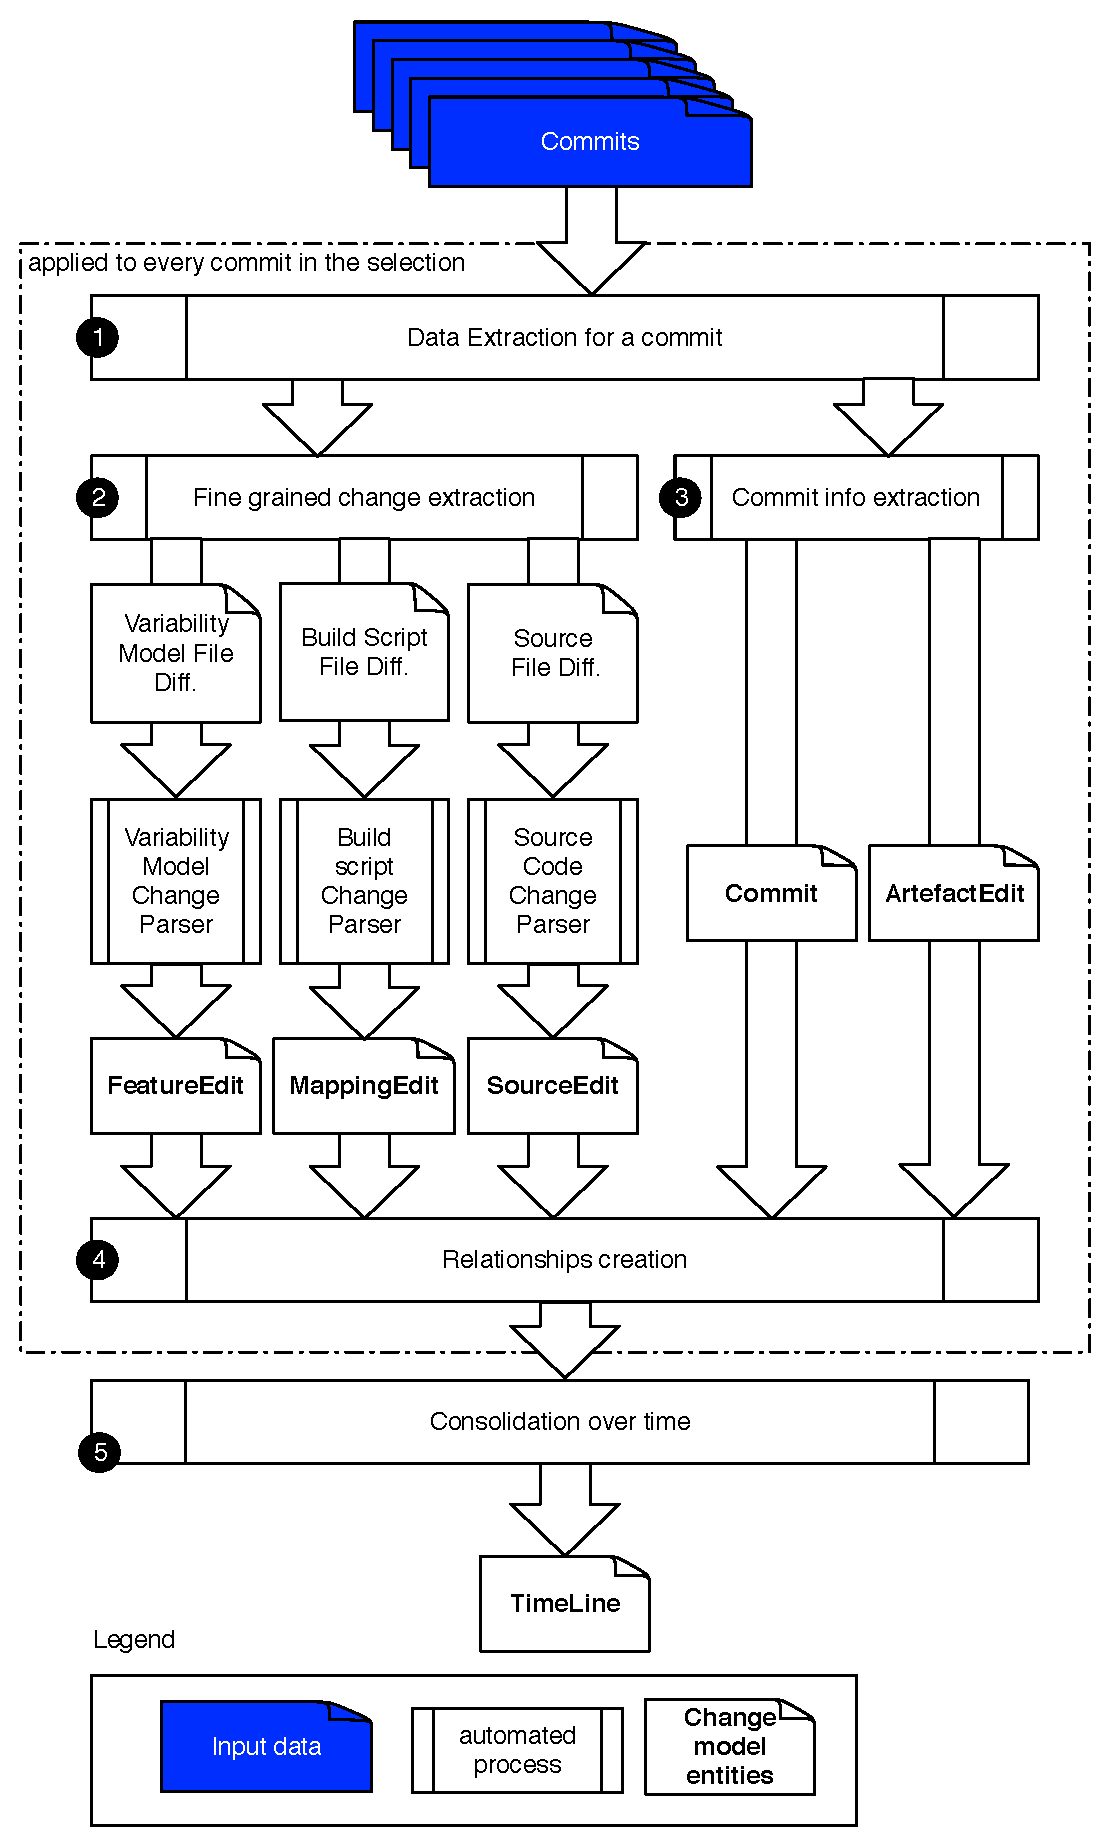
\includegraphics[scale=0.35]{extraction_overview.eps}
	\caption{Overview of the FEVER change extraction and consolidation process}
	\label{fig:overview}
\end{figure}
The FEVER approach starts from a set of commits and outputs an instance of the FEVER change model covering the given commit range.
\figref{fig:overview} presents an overview of the change extraction process.
From the initial set of commits, FEVER first analyses each commit separately, and then consolidates the extracted change information.
For each commit, Steps 1 to 4 are executed as follows:

\textit{Step 1} is the identification of the touched artefacts and the dispatch to the appropriate change parser.
In the Linux kernel, artefact types are characterized by naming conventions and file extensions using the mapping presented in \tabref{file_heuristics}.
Compared to our previous work \citep{dintzner_fever:_2016}, we adjusted our artefact identification heuristics regarding source files, with a more restrictive expression on ``.S'' files (rather than ``.S*'').
We also include binary files (libraries), which were previously not taken into account.

\begin{table}[h]
\centering
{
\begin{tabular}{|l|l|}
\hline
Artefact type & Expression used for identification\\
\hline
V.M. file	& ``Kconfig.*'' \\
Build file	& ``Makefile.*'',``Kbuild.*'',``Platform.*'' \\
Source file & ``*.c'', ``*.h'', ``*.s'', ``*.S''\\
Binary file & ``*.dll'',``*.so'',``*.a'',``*.lib''\\
Data file	& ``*.dts'',``*.dtb''\\
\hline
\end{tabular}
}
\caption{Artefact types: regular expression used to identify the different types of artefacts}
\label{file_heuristics}
\end{table}

\textit{Step 2} performs the artefact-specific data extraction processes. 
The next subsections (\secref{sec:vm_model},\secref{sec_mapping_model}, and \secref{sec_impl_model}) 
detail  the process for each type of artefact, but all of them follow the same general steps.
First FEVER rebuilds a model of the artefact as it was before the change, 
and a second one representing the same artefact after the change.
Then, FEVER uses the EMF Compare\footnote{\url{http://wiki.eclipse.org/EMF\_Compare}} infrastructure to identify 
the differences between the two versions of the model.
EMF Compare identifies the differences between the two models, and extracts them in terms of the EMF meta-model.
FEVER then translates those changes into the different \textbf{Edit} entities depending on the artefact type.
The reconstruction of the models, and the identification of changes (based on EMF Compare results)
are based on heuristics and assumptions on the structure of the artefacts.
We provide an evaluation of the accuracy of those heuristics in \secref{sec:evaluation}.

\textit{Step 3} is the extraction of changes in artefacts for which we do not extract detailed changes.
This includes only commit-related information from which we create a \textbf{commit} entity, 
and ``untyped'' artefacts (\ie documentation, or scripts), represented by \textbf{ArtefactEdit} entities.

In \textit{Step 4}, FEVER creates the relationships between \textbf{Edit} entities, the \textbf{Commit}, and \textbf{ArtefactEdit}.

\textit{Step 5} of our approach consists in creating entities and relationships spreading beyond single commits:
``next'' relationships among commits to keep track of the sequence of changes, and feature \textbf{TimeLine} entities 
with their respective relationships to edit entities.
This is done by navigating through every commit, and identifying touched feature(s), 
creating if necessary a new \textbf{TimeLine} entity and the appropriate relationships between 
the \textbf{TimeLine} and relevant edits.

We continue this section by describing the heuristics we used to extract feature related changes. 
Those heuristics are based on multiple sources of information, namely the work of Neves et al. \citep{neves_safe_2015}, the work of Passos et al. \citep{passos_coevolution_2015}, 
the Linux official documentation,  and finally the authors' expertise \citep{passos_coevolution_2015,dintzner_analysing_2015}.


\subsection{Extracting Variability Model Changes}
\label{sec:vm_model}

We describe in this section the artefact-specific change extraction process (Step 2 in \figref{fig:overview})
that takes place when a commit contains changes to the variability model of the system.
\begin{figure}[h]
	\centering
	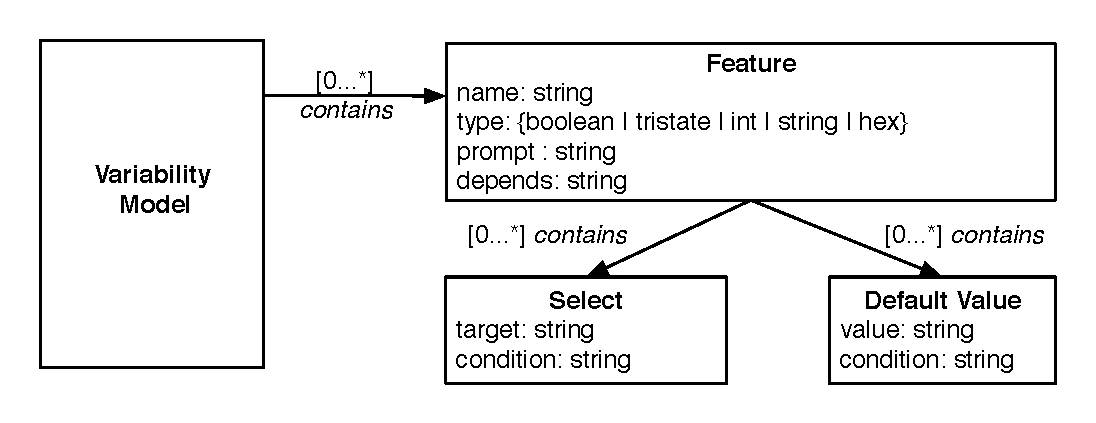
\includegraphics[scale=0.40]{EMF_VM_Model.eps}
	\caption{Representation of the variability model used for change extraction}
	\label{fig:vm_for_diff}
\end{figure}

The characteristics of the changed features that we focus on are their type (Boolean or value-based) and the change
affecting the feature.
We first reconstruct two instances of the VM depicted in \figref{fig:vm_for_diff} per VM file touched, 
one representing the VM before the change, the other after the change.
If, like in the case of the Linux kernel, the VM is described in multiple files,
we reconstruct the parts of the model described in the touched files, \ie the model we rebuild is always partial with respect to the complete Linux variability model.
The extraction process follows the FMDiff approach \citep{dintzner_analysing_2015}, including the usage of ``dumpconf''. 
This tool takes as an input a Kconfig file and translates it into XML. 
``dumpconf'' is designed to work on the complete Kconfig model, where the different files are linked together with a ``source'' statement, similar to \#include in C.
To invoke ``dumpconf'' successfully on isolated files, we remove the ``source'' statements as a pre-processing steps.
``dumpconf'' also affects the attributes of features, and the details of the change operation are described in \citep{dintzner_extracting_2013}.
We use this XML representation of the Linux VM to build the model shown in \figref{fig:vm_for_diff}.

We then use EMF Compare to extract the differences and compile the information in a \textbf{FeatureEdit} entity. 
To successfully compare two model instances, FEVER needs to provide EMF with the capability to determine that
two features in the two model instances are the same entity.
For this, we rely on the feature name as a unique identifier during the model comparison phase.

We attach to this entity the snapshot of the feature as it was before and after the change in \textbf{FeatureDesc} entities.
If the feature is new, respectively deleted, we do not create a ``before'', respectively ``after'', \textbf{FeatureDesc} entity.
As mentioned, the ``source'' statement in the Kconfig language is used to link Kconfig files together.
Such statements can be used in combination with other constructs, such as menus, or ``if'' blocks.
In this situation, the presence condition of the menu, or the condition of the ``if'' blocks, in practice
applies to all features within ``sourced'' file, and any of the files it might ``source'' itself.
By working on a file level (touched Kconfig file), FEVER will not capture such complex changes.

With respect to our previous work \citep{dintzner_fever:_2016}, we now handle cases where two features within the same file have the same name.
Whereas the previous heuristic yielded a number of false positive, such cases are now handled by suffixing feature names by an index if a feature name is encountered
twice (or more) when rebuilding the EMF model we use for change extraction.


\subsection{Extracting Mapping Changes}
\label{sec_mapping_model}

We describe in this section the artefact-specific change extraction process (Step 2 in \figref{fig:overview})
that takes place when a commit contains changes to the mapping between features and assets.

\begin{figure}[h]
	\centering
	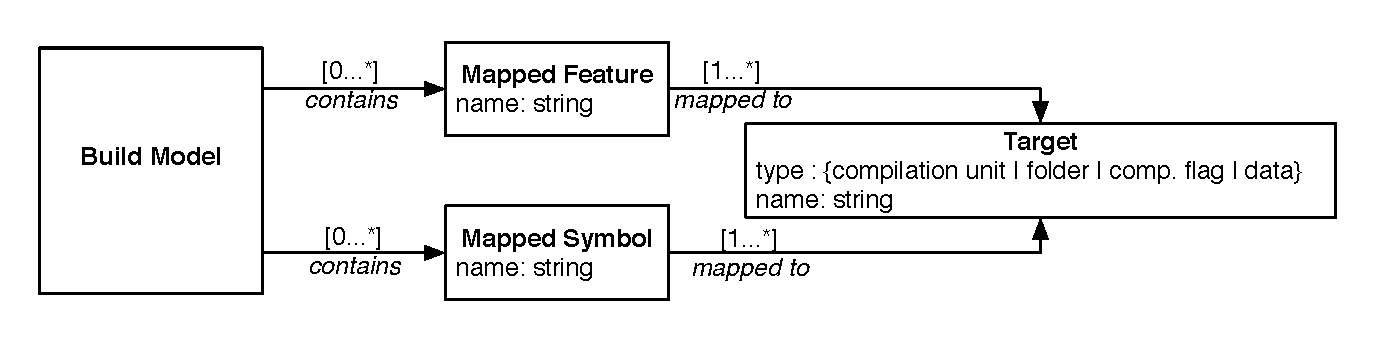
\includegraphics[scale=0.40]{EMF_Build_Model.eps}
	\caption{Representation of the feature-asset mapping used for change extraction}
	\label{fig:mapping_for_diff}
\end{figure}

Similar to the extraction of VM changes, \textbf{MappingEdit} entities are created based on the differences 
of reverse engineered models of a Makefile, before and after the change.
We use the model shown in \figref{fig:mapping_for_diff}.

The model contains a set of features and symbols mapped to targets. 
``Symbol'' refers to any variable mapped to any assets which is not a feature. 
We identify feature names in Makefiles by their prefix ``CONFIG\_''.
We scan the Makefiles and extract pairs of symbols by searching for assignment operators (``+='' and ``:=''). 
We consider that the symbol on the left hand side is mapped to the symbol on the right hand side (target).

To determine the type of a targeted asset, we use the following rules:
Compilation unit names finish with either ``.o'',``.c'' or ``.h''; 
mapped data artefacts in the Linux kernel are identified by the extensions ``.dts'', ``.dtb''; 
compilation flags either start by the follwing strings ``-D'', ``-L'', ``-m'',  or ``-W'', ``-I'', ``-f''.
We identify folder names by ``/'', or single words, not containing any special characters nor spaces.

Makefiles may contain lists of assets that will be included in the compilation 
as soon as the Makefile itself is included.
Those assets are assigned to Makefile variables whose names depend on the implementation of the build process.
In the Linux kernel, those are identified by \footnote{https://www.kernel.org/doc/Documentation/kbuild/makefiles.txt}:
``obj-y'',``lib-y'',``ccflags-y'',``asflags-y'', and ``ldflags-y''.
When we find assets associated with such variables, we map them to a temporary variable, using the following convention: we use the
key word ``guarded\_'' and append the name of folder containing the Makefile.
We later use this naming convention with the extracted information on features mapped to folders 
to assign the changes of such Makefile variables to the appropriate feature(s).

When features are found as part of ``ifeq'' or ``ifneq'' statements, we consider that they are mapped to any targets contained within their scope.
In Listing \ref{modular_makefile_ifdef}, both CONFIG\_OF and CONFIG\_SHDMA will be mapped to the compilation unit ``shdma.o''.

We also resolve aliases within Makefiles.
An example of an alias is presented in \listingref{modular_makefile_ifdef}, 
where feature CONFIG\_BLK\_DEV\_SWIM is mapped to the alias ``swim\_mod.o'' referring to two compilation units ``swim.o'' and ``swim\_asm.o''.
The association between ``swim\_mod'' and the two compilation units is done the last line of the listing.
We identify such aliases based on the naming convention : name of the object file appended by ``-y''.
Note that there are no concrete artefact corresponding to ``swim\_mod'' by itself in the Linux source tree.
This step is performed as a post-processing step for each build model instance, 
and is based on heuristics, also evaluated in \secref{sec:evaluation}.

\begin{lstlisting}[language=diff, caption=Example of an ``ifeq'' statement and aliases used in Makefiles, label=modular_makefile_ifdef]
ifeq ($(CONFIG_OF),y)
   shdma-$(CONFIG_SHDMA) += shdma.o
endif
obj-$(CONFIG_BLK_DEV_SWIM)	+= swim_mod.o
swim_mod-y	:= swim.o swim_asm.o
\end{lstlisting}

Finally, FEVER uses a Linux specific heuristic for mapping files contained within specific folders.
Part of the mapping between feature and folder is done using variable names, and dynamic path reconstruction.
In general, FEVER does not attempt to recover this mapping, but for a specific set of folder in the Linux kernel, namely the architecture folders,
this mapping is important.
Upon compilation, the chosen hardware architecture of the kernel forces the selection of a given subfolder of the ``./arch'' folder.
There is no explicit declarations of that mapping in any Makefile (it uses variables and name reconstruction).
For this reason, FEVER assumes that any file within the ``arch/x86'' folder maps to feature ``X86'' if no other mapping is found.
The accuracy of this heuristic to recover the link between features and artefacts is evaluated in the next section
as the \textit{feature-file mapping} change attribute.

Our model reconstruction is based on heuristics and therefor do not take into account all the possible constructs used in the Linux kernel to link artefacts to features, however, FEVER focuses on those mentioned above.
The constructs that FEVER does not capture are based on variable name manipulation, to build artefacts names (e.g. folder names, or file names),
or combining lists of artefacts together.
Then, as mentioned in \secref{sec:background}, the exact mapping between features and files
is the result of a complex Makefile hierarchy. 
By focusing on the mapping as described in a single Makefile, FEVER only captures a part of the presence condition
of each file.

Once the two instances of the model are reconstructed, we use EMF Compare to extract the differences between them,
giving us the list of feature mappings that were added or removed in that commit.
For the comparison of two instances of our mapping model, we use the name of features as unique identifiers.

From the earlier version of this work \citep{dintzner_fever:_2016}, we now capture mapping between features and more artefacts, and our coverage of compilation flags is more comprehensive.
In addition, we now take into account the changes to the mapped artefact as well. We can now determine whether a change in the mapping is also associated with changes to the mapped artefacts themselves. 
Doing so, we can differenciate cases where a feature change involves a new mapping to a new artefact, and cases where the new mapping points to a pre-existing artefact.


\subsection{Extracting Implementation Changes}
\label{sec_impl_model}

We describe in this section the artefact-specific change extraction process (Step 2 in \figref{fig:overview})
that takes place when a commit contains changes to the implementation (source code).

\begin{figure}[h]
	\centering
	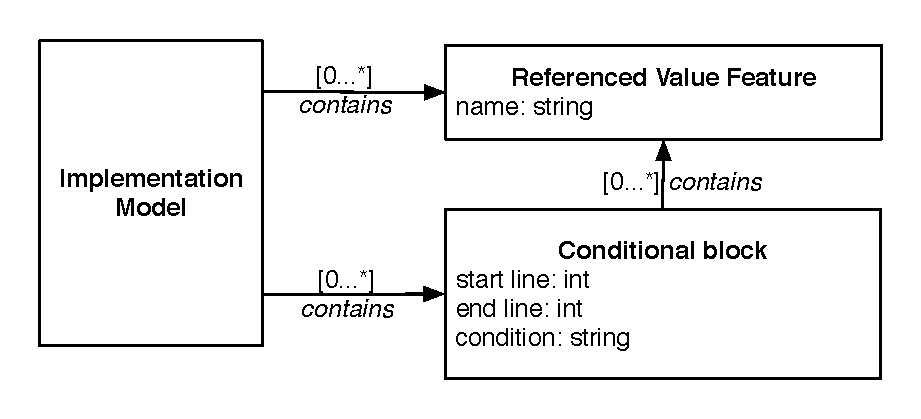
\includegraphics[scale=0.40]{EMF_Source_Model.eps}
	\caption{Representation of the feature-asset mapping used for change extraction}
	\label{fig:source_for_diff}
\end{figure}

At the implementation level, we consider changes to \#ifdef blocks and changes to feature references in the code, as presented in \secref{sec:background}.
To extract those changes, we rebuild a model of each implementation file in its before 
and after state following the model presented in \figref{fig:source_for_diff}.

To rebuild the models, we rely on CPPSTATS \citep{liebig_analysis_2010} to obtain 
starting and ending lines of each  \#ifdef block as well as their guarding condition. 
It should be noted that CPPSTATS provide the condition of each block by taking into account nesting.
In practice, if a block with condition B is nested inside a block with condition A, CPPSTATS will 
report two blocks, one with condition A and one with condition ``A\&B''.

In the model, code blocks and their \#else counter-parts are captured as two distinct entities.
``Referenced value features'' are obtained by scanning each modified source file looking for the usage 
of the ``CONFIG\_'' string outside of comments and \#ifdef statements.
Note that we report reference changes once per feature and per file.

We then use EMF Compare to compare the two models and build the \textbf{SourceEdit} entities.
For this comparison, FEVER needs to use a unique identifier for each code block contained within a source file. 
The condition on a block may not be unique, and hence cannot be used to uniquely identify a block in 
two versions of the source model.
The location of the block within the file may change during a commit without the block being changed itself
(\ie if code is added or removed above it).
FEVER uses a combination of the condition of the block combined with its content (the actual code)
as a unique identifier.
This proved to be an efficient technique, but in the context of the Linux kernel a number of files 
contain identical code blocks, with the same block condition.
While this may seem surprising, one may consider a logging mechanism: if the logger feature is selected, write an entry in the log file.
This might be repeated in multiple functions in a file. 
As a result, the EMF comparison process cannot correctly identify changed blocks and returns a number of false positive changes.
To compensate for this, we add indices to the identifier of code blocks when we find such duplication.

We determine the code changes occurring inside \#ifdef blocks to compute the value of the ``code edit'' attribute of 
\textbf{SourceEdit} entities.
This is performed as a separate step, once we found the changed code blocks.
We extract from the commit the diff of the file in the ``unified diff'' format, and identify which lines of code where modified.
We compare this information with the first and last lines of each modified code block to determine 
which code block is affected by the code changes.

FEVER extracts and records changes to all conditionally compiled code blocks - whether features play a role
in their presence condition or not.
Changes to code blocks that are not tied to any feature will be captured as \textbf{SourceEdit}, but
such entities will not be linked to any \textbf{TimeLine} in the next step of our process.

By comparison with our previous work \citep{dintzner_fever:_2016}, we enhance the source change extraction process by taking into account cases
where code artefacts contain identical code blocks, containing identical code. Such situations caused errors
during the EMF comparison process and are dealt with as explained in this section.


\subsection{Change Consolidation and TimeLines}
\label{sec:timelines}

The final step consists in the creation of feature \textbf{TimeLine} entities and relate them to the appropriate entities.
We create such entities for every feature touched affected by any change in any \textbf{Edit} entity.
We apply the following strategy: 
\begin{itemize}
\item if a feature is touched in the VM, mapping or source file, the corresponding \textbf{Edit} entity is associated with a \textbf{TimeLine} with a ``core update'' relationship.
\item if a feature A is added from another feature B's attribute (as part of a constraint), then the \textbf{FeatureEdit} entity representing this change is connected to the feature \textbf{TimeLine} with an ``influence update'' relationship if feature A did not participate at all in the definition of B before the change.
\item if a feature A is removed from another feature B's attribute (as part of a constraint), then the \textbf{FeatureEdit} entity representing this change is connected to the feature \textbf{TimeLine} with an ``influence update'' relationship if feature A no longer participate at all in the definition of B after the change.
\item if a feature is part of the condition in a \textbf{SourceEdit} entity, the \textbf{SourceEdit} is connected to one \textbf{TimeLine} entity per feature present in the condition with an ``influence update'' relationship;
\item if an artefact is touched, it is linked to the \textbf{TimeLine} entity of the feature to which it is mapped with a ``core update'' relationship. This is done for each feature mapped to the file.
\end{itemize}

In order to map file changes to features, we need to know the mapping between features and files.
Note that FEVER only focuses on mapping changes, leaving us with a gap with respect to mappings that are not touched.
As a result, many files, whose mapping has not evolved would not be mapped - wrongly - to any features.
To compensate for this, we create a snapshot of the complete mapping based on the state of the artefacts on the first commit of the commit set.
To support systems which do not follow Linux naming convention (the CONFIG\_ prefix used in Makefile and the source code), 
we also extract the list of features present at the beginning of the studied time-frame.
For both the initial feature list and initial mapping, 
we rely on the FEVER parser to obtain the information by invoking it for every Kconfig file and Makefile present in the system. 

We then run through all commits, starting from the leaves in a breadth-first manner, creating or updating \textbf{TimeLine} as necessary,
and updating the known mapping between files and features as we encounters \textbf{MappingEdits}.
Note that there may be more than one initial commit in a set: we have to consider branches as well. In our experiment we usually have
one initial commit of the release itself, and the different branches that have not yet been merged.\footnote{the list of commit is obtained using the following Git log command, asking for all commit reachable from the last considered commit and not accessible from the first commit of the release - i.e.: \textit{git log v3.7...v3.8}} 

Some files in the Linux kernel cannot be mapped directly to features. 
This concerns mostly header files, contained in ``include'' folders.
``Include'' folders do not contain Makefiles, which prevents direct mapping between features and such artefacts.
Moreover, such files are included in the compilation process on the basis that they are referenced by implementation files (\#include statement), 
which by definition bypasses any possible feature-related condition.
For those reasons, we do not attempt to map such files to features.
They are, however, highly conditional, and often contain many \#ifdef statements, which we track.
